\section{ВИЗУАЛИЗАЦИЯ ГРАФОВ}
Визуалиация была разработа с помощью
сторонней библиотеки <<matplotlib>>.

Для создания диаграмм графов был разработан класс
<<GraphPlotter>>. Данный клаcc содержит следущие поля:
\begin{enumerate}
    \item  <<graph>> -- граф, визуалиазация которого создается;
    \item <<coords>> -- словарь, где ключ -- это вершина, а значение
        координата;
    \item <<orange\_edges>> -- список ребер, которые 
        должны быть оранжевыми;
\end{enumerate}
\begin{figure}[H] 
\begin{lstlisting}[language=Python] 
    def __init__(self, g: Graph | GeoGraph | MultiGraph, orange_edges=[]):
        self.graph: Graph | GeoGraph | MultiGraph = g
        self.coords = {}
        self.gen_coords(g)
        self.orange_edges = orange_edges
\end{lstlisting}  
    \caption{Инициализация объекта типа <<GraphPlotter>>.}
\end{figure} 
Рассмотрим генерацию координат для 
вершины $v_{i}$
\begin{equation}
\begin{cases}
    r_{i} = \frac{2 \cdot i \cdot \pi }{n} \\
    x_{i} =  \cos{r_{i}}\\
    y_{i} = \sin{r_{i}}
\end{cases}
\label{coords}
\end{equation} 
Формула \ref{coords} задает укладку
вершин графа по окружности
\begin{figure}[H] 
\begin{lstlisting}[language=Python] 
    def __gen_coords(self, g: Graph | MultiGraph):
        for i, v in enumerate(g.verticies()):
            r = 2*i*pi / self.graph.k_vertecies()
            self.coords[v] = self.point(cos(r), sin(r))
\end{lstlisting}  
    \caption{Генерация словаря <<coords>>}
    \label{gcoors}
\end{figure} 
На риснуке \ref{gcoors} представлен метод для создания
координат вершин.
\begin{figure}[H] 
    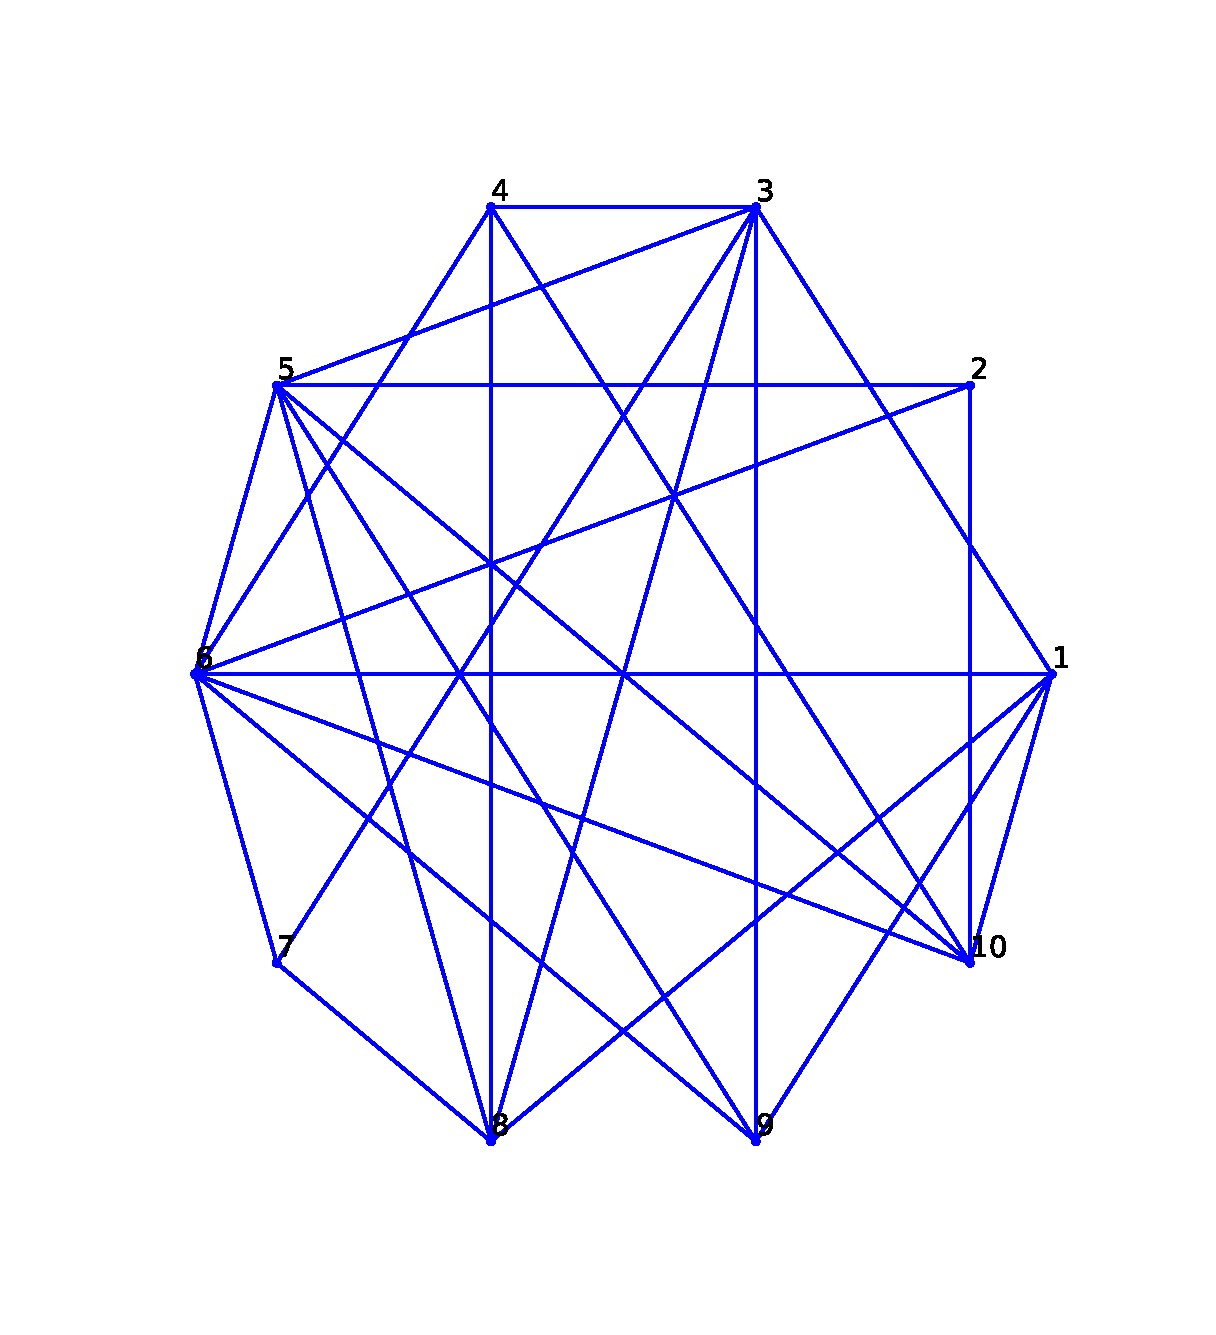
\includegraphics[scale=0.5]{g1.pdf}
    \caption{Пример диаграммы графа.}
    \label{gexp_1}
\end{figure} 
\begin{figure}[H] 
    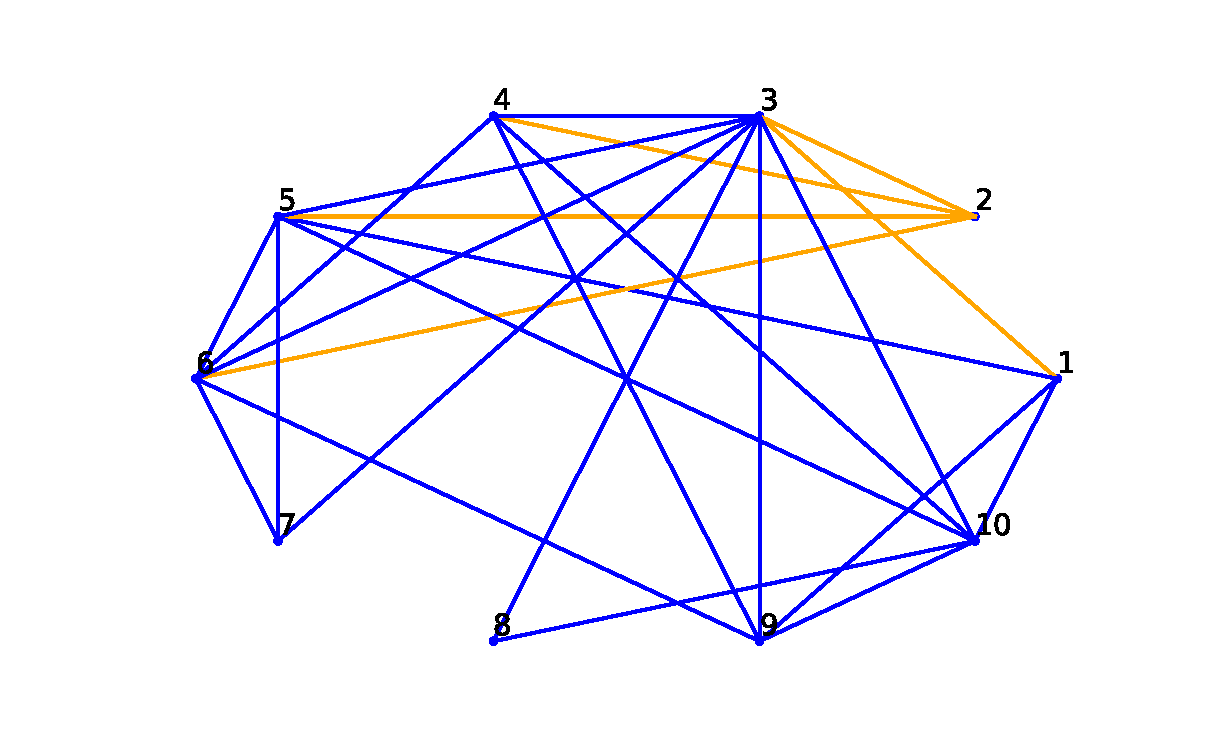
\includegraphics[scale=0.5]{g2.pdf}
    \caption{Пример диаграммы графа с оранжевыми ребрами.}
    \label{gexp_2}
\end{figure} 
На рисунках \ref{gexp_1}, \ref{gexp_2}
представлены диаграммы графов, созданные с помощью
<<GraphPlotter>>.
